\documentclass[border=12pt]{standalone}
\def\pgfsysdriver{pgfsys-dvisvgm.def}
\usepackage[dvisvgm]{xcolor}
\usepackage{xeCJK}
\setCJKmainfont{HaranoAjiGothic-Regular.otf}[BoldFont=HaranoAjiGothic-Bold.otf]
\setCJKsansfont{HaranoAjiGothic-Regular.otf}[BoldFont=HaranoAjiGothic-Bold.otf]
\usepackage{amsmath,amssymb,tikz,lmodern}
\usetikzlibrary{arrows.meta,positioning,calc}
\renewcommand{\familydefault}{\sfdefault}
\definecolor{ink}{HTML}{25322F}
\definecolor{green}{HTML}{246657}
\definecolor{tint}{HTML}{EEF4F0}
\definecolor{soft}{HTML}{C6D2CC}
\definecolor{muted}{HTML}{52615B}
\newif\ifJapanese
\newcommand{\Tx}[2]{\ifJapanese #1\else #2\fi}
\newcommand{\heading}[3]{{\color{green}\bfseries #1\quad\Tx{#2}{#3}}\\[5pt]}
\newcommand{\Var}{\operatorname{Var}}
\newcommand{\Frac}{\operatorname{Frac}}
\newcommand{\C}{\mathbb C}
\newcommand{\refurl}[2]{\special{dvisvgm:raw <a xlink:href="#1" target="_blank" rel="noopener noreferrer">}{\setlength{\fboxsep}{0pt}\colorbox{white}{\color{green}\underline{\strut #2}}}\special{dvisvgm:raw </a>}}
\newcommand{\R}[2]{\refurl{\csname source#1\endcsname}{#2}}
\tikzset{
 card/.style={draw=soft,fill=white,rounded corners=2pt,align=left,text=ink,font=\fontsize{10.5}{14}\selectfont,inner xsep=12pt,inner ysep=11pt,text width=14.4cm},
 result/.style={card,draw=green,fill=tint,line width=.9pt},
 reason/.style={align=left,text=muted,font=\fontsize{9}{12}\selectfont,inner sep=0pt,text width=12.7cm},
 edge/.style={-{Stealth[length=2.4mm]},draw=green,line width=1pt}
}
\newcommand{\flow}[3]{
 \coordinate (#2-from) at ($(#1.south)+(-6.9,0)$);
 \coordinate (#2-to) at ($(#2.north)+(-6.9,0)$);
 \draw[edge] (#2-from)--(#2-to);
 \node[reason,anchor=west] at ($(#2-from)!.5!(#2-to)+(.55,0)$) {#3};
}

\Japanesetrue
\expandafter\def\csname sourceWV\endcsname{https://github.com/openai/math/blob/fd4aeeb2ee4fc729c18d98444fed42fd0529eeeb/preprints/Logarithmic-Kodaira-dimension-and-whole-fiber-variation-September-26-2026/paper.pdf}
\expandafter\def\csname sourceOI\endcsname{https://github.com/openai/math/blob/fd4aeeb2ee4fc729c18d98444fed42fd0529eeeb/preprints/Orbifold-and-logarithmic-Iitaka-subadditivity-September-26-2026/paper.pdf}
\expandafter\def\csname sourcePH\endcsname{https://github.com/openai/math/blob/fd4aeeb2ee4fc729c18d98444fed42fd0529eeeb/preprints/Projective-Hodge-lines-and-ordinary-Iitaka-subadditivity-September-27-2026/paper.pdf}
\expandafter\def\csname sourceRA\endcsname{https://github.com/openai/math/blob/fd4aeeb2ee4fc729c18d98444fed42fd0529eeeb/preprints/The-reverse-logarithmic-Kodaira-inequality-and-additivity-September-26-2026/paper.pdf}
\expandafter\def\csname sourceLA\endcsname{https://github.com/openai/math/blob/adc7f1241b42e322a6451854ab7e4b4c146bf78a/preprints/Log-abundance-in-characteristic-zero-September-24-2026/paper.pdf}
\expandafter\def\csname sourceFuj\endcsname{https://www.math.kyoto-u.ac.jp/~fujino/weak-posi11.pdf}
\expandafter\def\csname sourceDel\endcsname{https://www.numdam.org/item/PMIHES_1971__40__5_0.pdf}
\expandafter\def\csname sourceDHP\endcsname{https://arxiv.org/pdf/1012.0493v2}
\expandafter\def\csname sourcePT\endcsname{https://arxiv.org/pdf/1409.5504v1}
\expandafter\def\csname sourceBCHM\endcsname{https://arxiv.org/pdf/math/0610203v2}
\expandafter\def\csname sourceKP\endcsname{https://sites.math.washington.edu/~kovacs/2013/papers/Kovacs_Patakfalvi__Projectivity.pdf}
\expandafter\def\csname sourceHan\endcsname{https://doi.org/10.1007/BF01394338}
\expandafter\def\csname sourceSGA1\endcsname{https://arxiv.org/abs/math/0206203v2}
\expandafter\def\csname sourceLan\endcsname{https://arxiv.org/pdf/2005.09690v3}
\expandafter\def\csname sourceBDPP\endcsname{https://arxiv.org/pdf/math/0405285v1}
\expandafter\def\csname sourceTaj\endcsname{https://arxiv.org/pdf/2005.01025v4}
\begin{document}
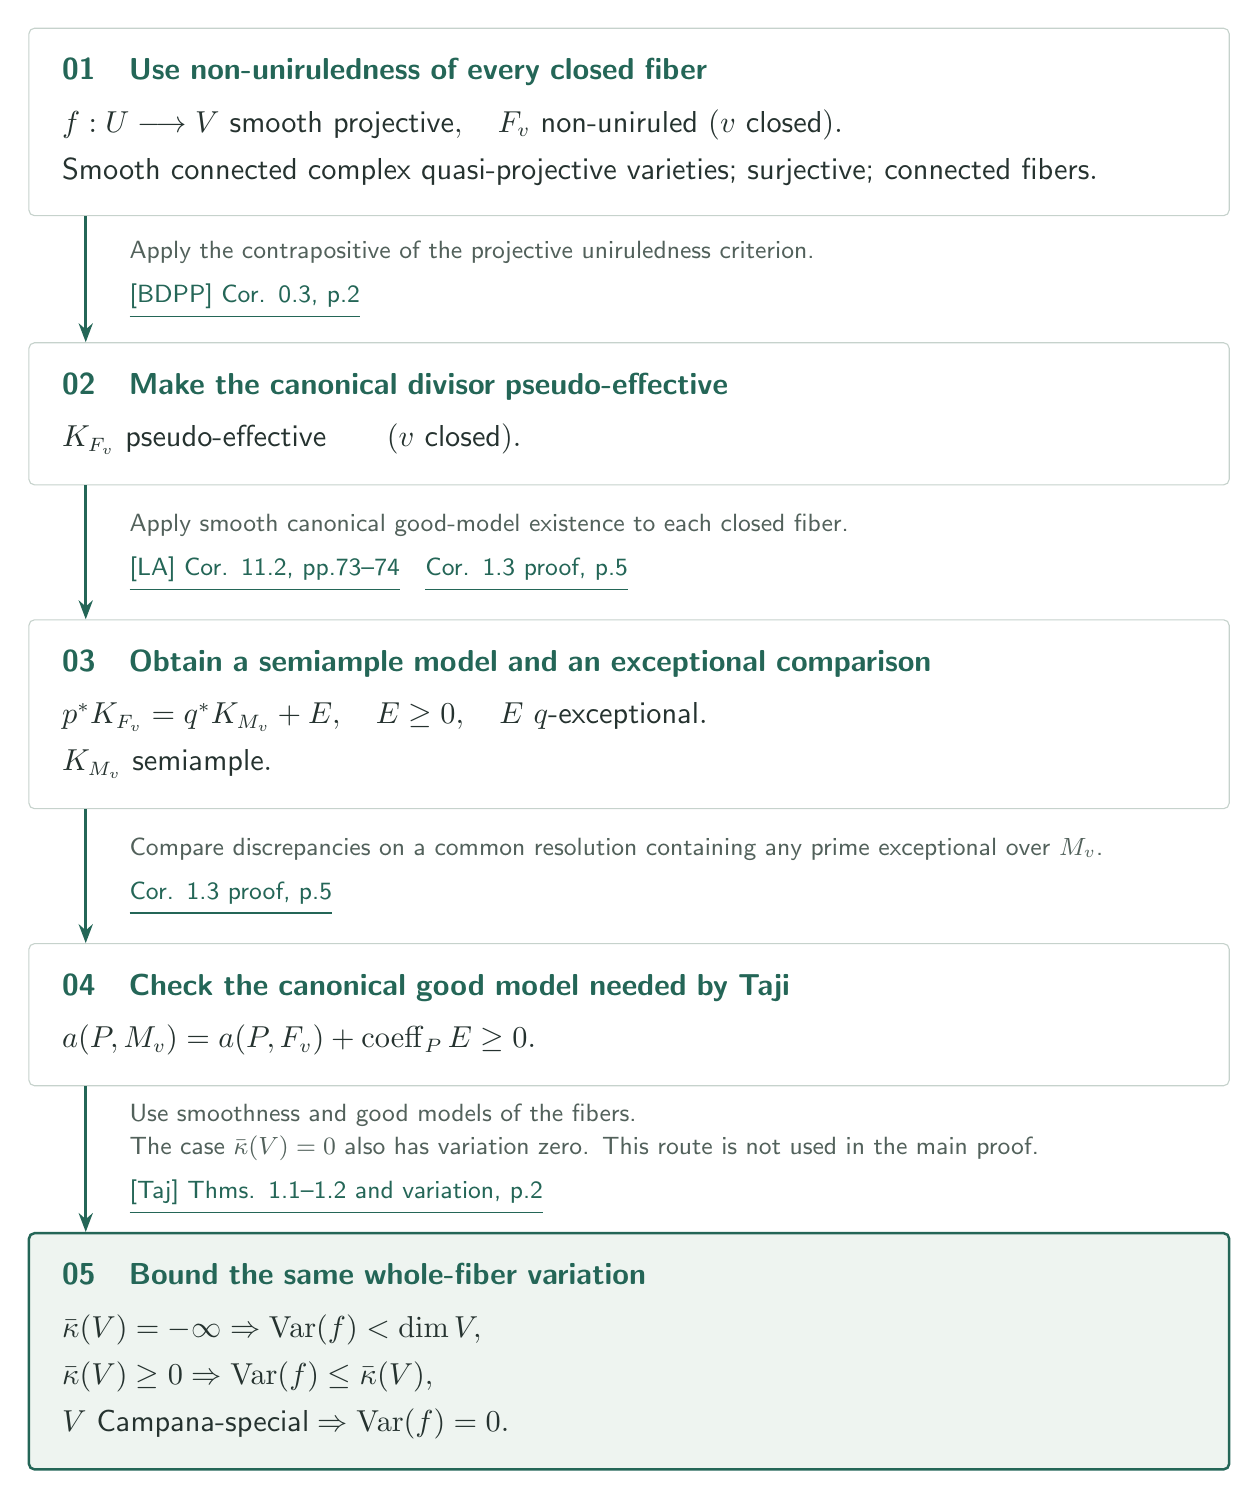
\begin{tikzpicture}
\node[card] (input) {\heading{01}{すべての閉ファイバーのnon-unirulednessを使う}{Use non-uniruledness of every closed fiber}
$f:U\longrightarrow V\ \text{smooth projective},\quad F_v\ \text{non-uniruled}\ (v\text{ closed}).$\\[3pt]
$\Tx{\text{滑らかな連結複素準射影多様体、全射、連結ファイバー}}{\text{Smooth connected complex quasi-projective varieties; surjective; connected fibers}}.$};
\node[card,below=1.6cm of input] (pe) {\heading{02}{標準因子をpseudo-effectiveにする}{Make the canonical divisor pseudo-effective}
$K_{F_v}\ \text{pseudo-effective}\qquad(v\text{ closed}).$};
\flow{input}{pe}{\Tx{射影多様体に対するuniruledness判定の対偶を使う。}{Apply the contrapositive of the projective uniruledness criterion.}\\[4pt]
\R{BDPP}{[BDPP] Cor. 0.3, p.2}}
\node[card,below=1.7cm of pe] (good) {\heading{03}{semiampleなモデルと例外項の比較式を得る}{Obtain a semiample model and an exceptional comparison}
$p^*K_{F_v}=q^*K_{M_v}+E,\quad E\ge0,\quad E\ \text{$q$-exceptional}.$\\[3pt]
$K_{M_v}\ \text{semiample}.$};
\flow{pe}{good}{\Tx{smooth canonical good-modelの存在定理を各閉ファイバーへ適用。}{Apply smooth canonical good-model existence to each closed fiber.}\\[4pt]
\R{LA}{[LA] Cor. 11.2, pp.73--74}\quad\R{WV}{Cor. 1.3 proof, p.5}}
\node[card,below=1.7cm of good] (canonical) {\heading{04}{Tajiに必要なcanonicalなgood modelを確認する}{Check the canonical good model needed by Taji}
$a(P,M_v)=a(P,F_v)+\operatorname{coeff}_P E\ge0.$};
\flow{good}{canonical}{\Tx{任意の $M_v$-exceptional因子を含む共通解消でdiscrepancyを比較。}{Compare discrepancies on a common resolution containing any prime exceptional over $M_v$.}\\[4pt]
\R{WV}{Cor. 1.3 proof, p.5}}
\node[result,below=1.85cm of canonical] (bounds) {\heading{05}{同じwhole-fiber variationの上界を得る}{Bound the same whole-fiber variation}
$\bar\kappa(V)=-\infty\Rightarrow\Var(f)<\dim V,$\\[3pt]
$\bar\kappa(V)\ge0\Rightarrow\Var(f)\le\bar\kappa(V),$\\[3pt]
$V\ \text{Campana-special}\Rightarrow\Var(f)=0.$};
\flow{canonical}{bounds}{\Tx{smooth familyと各ファイバーのgood modelを入力する。\\$\bar\kappa(V)=0$ でもvariationは0。主定理の証明には用いない。}{Use smoothness and good models of the fibers.\\The case $\bar\kappa(V)=0$ also has variation zero. This route is not used in the main proof.}\\[4pt]
\R{Taj}{[Taj] Thms. 1.1--1.2 and variation, p.2}}
\end{tikzpicture}

\end{document}
